\documentclass[12pt]{report}

%IMPORTS
\usepackage[catalan]{babel}
\usepackage[utf8]{inputenc}
\usepackage{graphicx}
\usepackage{wrapfig}
\usepackage{amsmath}
\usepackage{amssymb}
\usepackage{ragged2e} 
\usepackage{subfig}
\usepackage{caption}
\usepackage{subcaption}
\usepackage[usenames]{color}
\usepackage{xcolor}
\usepackage{float}
\usepackage{chngcntr}
\usepackage{ragged2e}
\usepackage{multirow}
\usepackage{vmargin}
\usepackage{hyperref}
\usepackage{url}
\usepackage{bigints}
\usepackage{listings}
\usepackage{amsmath}

\definecolor{navy}{rgb}{0,0,128}

\setpapersize{A4}
\setmargins{2.5cm}     % margen izquierdo
{2.6cm}                % margen superior
{16.5cm}               % anchura del texto
{23.7cm}               % altura del texto
{10pt}                 % altura de los encabezados
{0cm}                  % espacio entre el texto y los encabezados
{0pt}                  % altura del pie de página
{1cm}                  % espacio entre el texto y el pie de página
\renewcommand{\baselinestretch}{1.5}

\begin{document}

\begin{titlepage}
    \centering
    {\bfseries\LARGE Universitat Autònoma de Barcelona\newline Facultat de Ciències\par}
    \vspace{2cm}
    {\hspace{-1em}\includegraphics[width=0.4\textwidth]{}\par}
    \vspace{1cm}
    {\scshape\Huge Lliurament Equip 5 \par} 
    \vspace{1cm}
    {\Large \itshape Autors: \par}
    {\large Gerard Lahuerta 1601350\par}
    {\large Ona Sánchez 1601181 \par}
    {\large Pau Ventura 1601350 \par}
    \vspace{1cm}
    {\Large 11 de Juny del 2021\par}
\end{titlepage}

\justifying


\newpage
\setcounter{page}{2}
\pagestyle{plain}
\tableofcontents
\cleardoublepage
\addcontentsline{}{chapter}{}




\chapter{Exercici 1}
\section{Enunciat}
Trobar el polinomi de grau 3 associat a una funció $f: \mathbb{R}^2 \to \mathbb{R}$ que compleix les igualtats següents:
\begin{itemize}
    \item [$\bullet$] $ f(-5,3)=-24 $
    \item [$\bullet$] $ f(0,2)=17 $
    \item [$\bullet$] $ \frac{\partial f}{\partial y}(0,0) =4 $
    \item [$\bullet$] $ \frac{\partial^2 f}{\partial y^2}(1,1) = \frac{\partial f}{\partial x \partial y}(-2,3) = 2 $
    \item [$\bullet$] $ D_{(0,-1)}f(2,2)=-12 $
    \item [$\bullet$] $ D_{(-1/\sqrt{2},-1/\sqrt{2})}f(-3,0)= \frac{-1}{\sqrt{2}} $
    \item [$\bullet$] $ D_{(0,1)}f(3,6)=22 $
    \item [$\bullet$] $ D_{(-1/\sqrt{2},1/\sqrt{2})}f(-4,0)=\frac{-80}{\sqrt{2}} $
    \item [$\bullet$] $ \frac{\partial f}{\partial x}(-1,0) - 2\frac{\partial f}{\partial y}(0,0) =-7 $
    \item [$\bullet$] $ D_{(1/\sqrt{2},1/\sqrt{2})}f(-2,0)=0 $
\end{itemize}
\section{Procediment}
Vam utilitzar el sagemath per a interpolar el polinomi imposant totes les restriccions que ens donava l'enunciat, creant una matriu (A) amb els coeficients de les incógnites, i un vector (b) amb les solucions de les equacions. 
\newline
Al final vam tenir que resoldre un sistema de la forma:
\[Ax = b \]
On x són els coeficients, és a dir, les incógnites.
\section{Solució}

\begin{center}
    $f(x, y) = x^{3}+5x^{2}+2xy+y^{2}+4x+4y+5$
\end{center}


\chapter{Exercici 2}
\section{Enunciat}
Considerem les regions planes següents:

\[ \Omega_1 = {(x,y) : \frac{1}{2} \le x^2 + y^2 \le 5, y \ge |x| }\]
\[ \Omega_2 = {(x,y) : 0 \le x \le 1, x \le 3y \le (x^2+5), 0\le x \le 1 }\]

Calculeu la integral de la vostra funció sobre cadascuna d'aquestes regions. Per a la integral sobre la segona regió, calculeu la integral en els dos possibles ordres d'integració i comproveu que obteniu el mateix resultat.
\newpage
\section{Procediment}
\begin{center}
    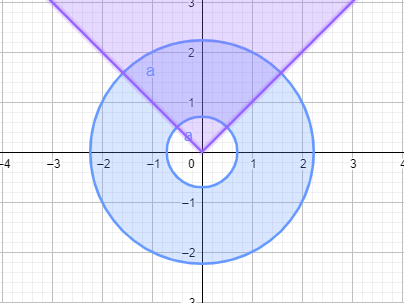
\includegraphics[width=0.404\textwidth]{regio_plana1.PNG}
    \label{$\Omega_1$}
    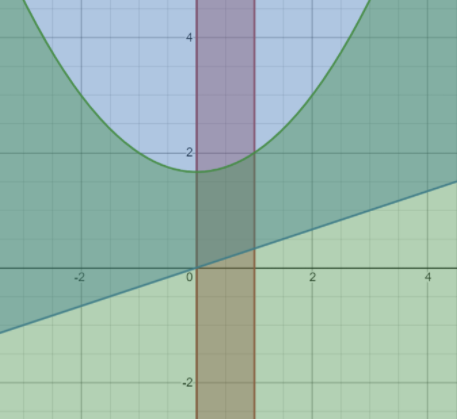
\includegraphics[width=0.33\textwidth]{regio_plana2.PNG}
\end{center}
 \text{\hspace{12.5em} $\Omega_1$\hspace{13.35em} $\Omega_2$}

\subsection{Calculem l'area definida sobre $\Omega_1$}

Volem trobar:
\[\int\int_{\Omega_1} f(x,y)\ dxdy = \int\int_{\Omega_1} x^{3}+5x^{2}+2xy+y^{2}+4x+4y+5\  dxdy \]
Com que és un cercle, ens interessa fer el cànvi a coordenades polars:
\begin{equation*}
    \left\{
    x = rcos(\theta) \atop
    y = rsin(\theta) \right.
\end{equation*}
Amb $J\phi = r$\newline
Així doncs:
\begin{gather*}
    \int_{ \frac{\pi}{4} }^{\frac{3\pi}{4}} \! \int_{\frac{1}{\sqrt{2}}}^{\sqrt{5}} \! \scriptstyle r((rcos(\theta))^3+5(rcos(\theta))^2+2rcos(\theta)rsin(\theta)+(rsin(\theta))^2+4(rcos(\theta) + 4(rsin(\theta)) + 5 )drd\theta =
\end{gather*}
\begin{gather*}
\int_{\frac{\pi}{4}}^{\frac{3\pi}{4}} \!  \left(\scriptscriptstyle  297\cdot \sqrt{2^5} \cdot \sin^2{x} + 297\cdot \sqrt{2^7} \cdot \cos{x} + (\sqrt{2^21 \cdot 5^3}-512) \sin{x} + (\sqrt{2^13 \cdot 5^3} -32) \cos^3{x} +1485 \cdot \sqrt{2^5} \cos^2{x} + (\sqrt{2^17\cdot 5^3} -128)\cos{x} + \frac{135}{3} \right) d\theta =
\end{gather*}
\begin{gather*}
    = 169.12947 \Rightarrow \fcolorbox{black}{white}{$\int\int_{\Omega_1} f(x,y)dxdy \approx 169.12947 u^2$}
\end{gather*}
% 169.12947
\newpage
\subsection{Calculem l'area definida sobre $\Omega_2$}
Volem trobar:
\[\int\int_{\Omega_2} f(x,y)\ dxdy = \int\int_{\Omega_2} x^{3}+5x^{2}+2xy+y^{2}+4x+4y+5\  dxdy \]

\subsubsection{Primer ordre}
Definint els límits d'integració:
\[\int_{0}^{1}\int^{\frac{x^2+5}{3}}_{\frac{x}{3}} x^{3}+5x^{2}+2xy+y^{2}+4x+4y+5\  dydx =\]
\[=\int_{0}^{1} \frac{x^6 + 36x^5 + 141x^4 + 188x^3 + 939x^2 + 630x + 1250}{81} dx = \]
\[=\left[ \frac{x ( 5x^6 + 210x^5 + 987x^4 + 1645x^3 + 10955x^2 + 11025x + 43750}{2835}\right]_{0}^1 = \]
\begin{equation*}
    = \frac{22859}{945} \approx 24.18 u^2 \Rightarrow \fcolorbox{black}{white}{$\int\int_{\Omega_2} f(x,y)dxdy \approx 24.18 u^2$}
\end{equation*}

\subsubsection{Segón ordre}
\[\int_{0}^{\frac{1}{3}}\int_{0}^{3y} f(x,y)\ dxdy + \int_{\frac{1}{3}}^{\frac{5}{3}}\int_{1}^{0} f(x,y)\ dxdy+ \int_{\frac{3}{5}}^{2}\int_{\sqrt{3y-5}}^{1} f(x,y)\ dxdy \]

Calculem la primera integral:

\[\int_{0}^{\frac{1}{3}}\int_{0}^{3y} f(x,y)\ dxdy = 
\int_{0}^{\frac{1}{3}}\int_{0}^{3y} x^{3}+5x^{2}+2xy+y^{2}+4x+4y+5\ dxdy = \]
\[=\int_{0}^{\frac{1}{3}} \frac{81y^4+228y^3+120y^2+60y}{4} dy = \left[ \frac{y^2(81y^3 + 285y^2 + 200y + 150)}{20} \right]_{0}^\frac{1}{3} = \]
\[= \frac{377}{270} \approx 1.39 \]

Calculem la segona integral:

\[ \int_{\frac{1}{3}}^{\frac{5}{3}}\int_{1}^{0} f(x,y)\ dxdy = \int_{\frac{1}{3}}^{\frac{5}{3}}\int_{1}^{0} x^{3}+5x^{2}+2xy+y^{2}+4x+4y+5\ dxdy =\]
\[= \int_{\frac{1}{3}}^{\frac{5}{3}}\frac{12y^2+60y+107}{12}dy = \left[ \frac{y(4y^2+30y+107)}{12}\right]^{{\frac{5}{3}}}_{\frac{1}{3}}= \frac{1627}{81} \approx 20.08\]

Calculem la tercera integral:
\[\int_{\frac{5}{3}}^{2}\int_{\sqrt{3y-5}}^{1} f(x,y)\ dxdy = \int_{\frac{5}{3}}^{2}\int_{\sqrt{3y-5}}^{1} x^{3}+5x^{2}+2xy+y^{2}+4x+4y+5\ dxdy = \]
\[=\int_{\frac{5}{3}}^{2} -\frac{\sqrt{3y-5}(12y^2+108y-40) + 51y^2 - 138y -152}{12}dy = \frac{15347}{5670} \approx 2.70 \]

Així doncs, en total:
\[\int_{0}^{\frac{1}{3}}\int_{0}^{3y} f(x,y)\ dxdy + \int_{\frac{1}{3}}^{\frac{5}{3}}\int_{1}^{0} f(x,y)\ dxdy+ \int_{\frac{3}{5}}^{2}\int_{\sqrt{3y-5}}^{1} f(x,y)\ dxdy =  \]
\begin{equation*}
    = 1.39 + 20.08 + 2.7 \approx 24.18 \Rightarrow \fcolorbox{black}{white}{$\int\int_{\Omega_2} f(x,y)dxdy \approx 24.18 u^2$}
\end{equation*}
% \begin{figure}
%     \centering
%     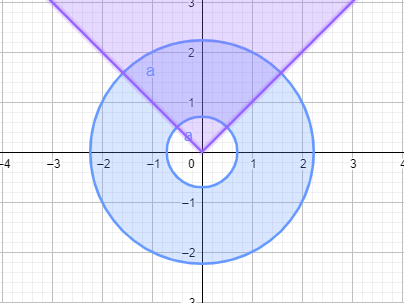
\includegraphics[width=0.42\textwidth]{regio_plana1}
%     \caption{$\Omega_1$ }
%     \label{fig:omega1-ex2}

%     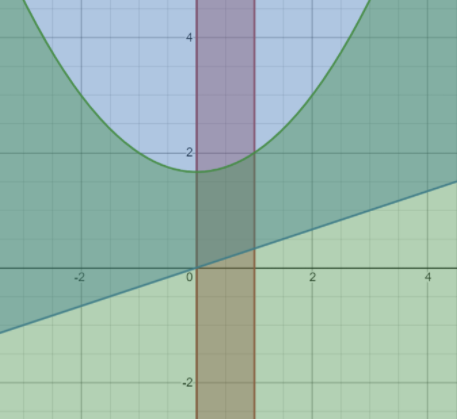
\includegraphics[width=0.3435\textwidth]{regio_plana2}
%     \caption{$\Omega_2$ }
%     \label{fig:omega1-ex2}
    
% \end{figure}
% $\Omega$_2: 
% 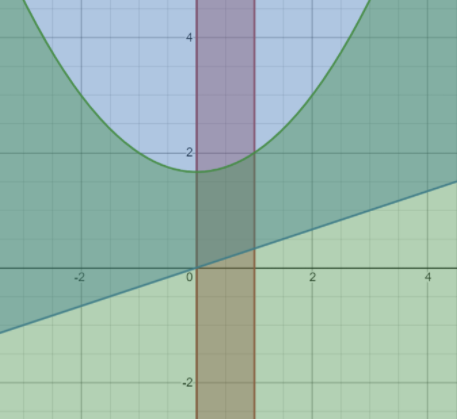
\includegraphics[width=0.3435\textwidth]{regio_plana2}

\section{Solució}
El resultat de la funció definida sobre $\Omega_1$ és 756.42$u^2$.
\newline
El resultat de la funció definida sobre $\Omega_2$ és 24.18$u^2$, i s'ha corroborat mitjançant el càlcul amb diversos mètodes.


\chapter{Exercici 3}
\section{Enunciat}
Determineu els extrems relatius de \textit{f} i classifiqueu-los.

\section{Procediment}

\subsection{Busquem els punts crítics}
Els punts crítics són:
\[ \{(a,b) : \nabla f(a,b) = 0\} \]\
Calculem el gradient en un punt general:
\[  \nabla f(x,y) = (3x^2+10x+2y+4, 2x+2y+4) \]
Llavors només cal resoldre el sístema:

\begin{equation*}
    \left.
    3x^2+10x+2y+4=0 \atop
    2x+2y+4=0 \right\}
\end{equation*}

On les solucions són:
\[(x,y) = (0,-2) \]
\[(x,y) = \left(\frac{-8}{3},\frac{2}{3}\right) \]
 
 
\subsection{Calculem la matriu Hessiana}


\[H(x,y) =
\begin{pmatrix}
    6x+10 & 2 \\
    2 & 2
\end{pmatrix} 
\]

\subsection{Avaluem la matriu Hessiana en els punts crítics i calculem el determinant}
\textcolor{white}{hola}\\
$\left.
\begin{array}{ccccccc}
    H(0,-2) & = & \begin{pmatrix}
                    10 & 2 \\
                    2 & 2
                  \end{pmatrix} & \Rightarrow  &|H(0,-2)| & = & 16 \\
                  \\
    H\left(\frac{-8}{3},\frac{2}{3}\right) & = &
     \begin{pmatrix}
        -6 & 2 \\
         2 & 2
    \end{pmatrix} & \Rightarrow & |H\left(\frac{-8}{3},\frac{2}{3}\right)| & = & -16\\
\end{array}\right\}\Rightarrow \begin{array}{cc}
    \text{El mínim relatiu és} & (0,-2). \\
    \text{El punt de sella és} & \left(\frac{-8}{3},\frac{2}{3}\right).
\end{array}$




\section{Solució}
\begin{wrapfigure}{l}{0.5\textwidth}
    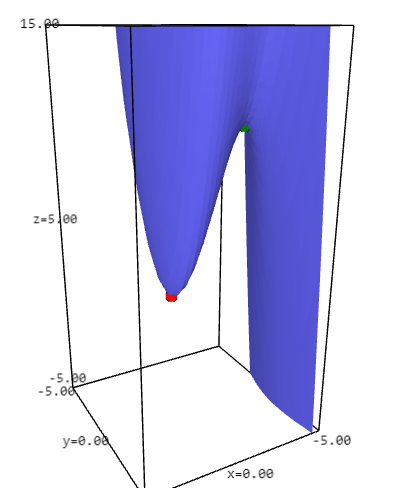
\includegraphics[width=0.5\textwidth]{image.PNG}
    \label{$Roig: (0,-2). Verd:(-8/3, 2/3)$}
\end{wrapfigure}
\textcolor{white}{hola}
\newline
\newline
\newline
\newline
Per al punt (x,y) = (0,-2), com que el determinant és positiu i el terme $A_1$(10) també ho és, el punt es tractarà d'un \textbf{mínim} (representat en roig). \newline\newline
Per al punt (x,y) = $\left(\frac{-8}{3},\frac{2}{3}\right)$, com que el determinant és negatiu, el punt es tractarà d'un \textbf{punt de sella} (representat en verd). 


\chapter{Exercici 4}
\section{Enunciat}
Sigui \textit{K} el quadrilàter (amb interior) limitat per les rectes $-4y +2x = \pm 1$ i $3x + 2y = \pm 4$.
Quin és el valor més gran que pren \textit{f} sobre \textit{K}? I el més petit?

\section{Procediment}

Fem la representació del quadrilàter:

\begin{center}
    \includegraphics[width=0.7\textwidth]{quadrilàter.PNG}
\end{center}


Al ser un conjunt plè, cal fer l'estudi de:
\begin{enumerate}
    \item L'interior del conjunt.
    \item La frontera del conjunt.
    \item Els punts de conjunció de la frontera.
\end{enumerate}

\subsection{L'interior del conjunt}
Com hem vist a l'apartat 3, els punts crítics corresponents als extrems relatius de la funció es troben fora del conjunt que estem tractant, així que si hi ha mínims i màxims es trobaran a la frontera.


\subsection{La frontera del conjunt}
Per a estudiar la frontera del conjunt estudiarem per separat els punts crítics de les rectes mitjançant el teorema de Multiplicadors de Lagrange.
 
Així doncs, per a cada recta $g(x,y)$, hem de trobar els punts (a,b) que compleixin:
\[\nabla f(a,b) = \lambda \nabla g(a,b)\]
\[\ g(a,b) = 0\]

Les posibles solucions resultants són:\\
Recta 1:\\
\hspace{5em} $\begin{array}{ccc}
    x = \frac{1}{12}\sqrt{301} - \frac{25}{12} & ; & y = \frac{1}{24}\sqrt{301} - \frac{19}{24} \\
    x = \frac{-1}{12}\sqrt{301} - \frac{25}{12} & ; & y = \frac{-1}{24}\sqrt{301} - \frac{19}{24}
\end{array}$\\
Recta 2:\\
\hspace{5em} $\begin{array}{ccc}
    x = \frac{1}{12}\sqrt{373} - \frac{25}{12} & ; & y = \frac{1}{24}\sqrt{373} - \frac{31}{24}\\
    x = \frac{-1}{12}\sqrt{373} - \frac{25}{12} & ; & y = \frac{-1}{24}\sqrt{373} - \frac{31}{24}
\end{array}$\\
Recta 3:\\
\hspace{5em} $\begin{array}{ccc}
    x = \frac{1}{12}\sqrt{481} - \frac{17}{12} & ; & y = \frac{-1}{8}\sqrt{481} - \frac{33}{8}\\
    x = \frac{-1}{12}\sqrt{481} - \frac{17}{12} & ; & y = \frac{1}{8}\sqrt{481} - \frac{33}{8}
\end{array}$\\
Recta 4:\\
\hspace{5em} $\begin{array}{ccc}
    x = 0 & ; & y = -2\\
    x = \frac{-17}{6} & ; & y = \frac{9}{4}
\end{array}$
\newline
D'aquestes possibles solucions, pertanyen al quadrilàter només:\\
x = $\frac{1}{12}\sqrt{301}$ - $\frac{25}{12}$ ; y = $\frac{1}{24}\sqrt{301}$ - $\frac{19}{24}$\\
x = $\frac{1}{12}\sqrt{373}$ - $\frac{25}{12}$ ; y = $\frac{1}{24}\sqrt{373}$ - $\frac{31}{24}$\\

Amb imàtges:
\[f\left(\frac{1}{12}\sqrt{301} - \frac{25}{12},\frac{1}{24}\sqrt{301} - \frac{19}{24} \right) = 4.04\]
\[f\left(\frac{1}{12}\sqrt{373} - \frac{25}{12}, \frac{1}{24}\sqrt{373} - \frac{31}{24} \right) = 2.87\]

Així doncs, podem concloure que el primer punt és el màxim dels punts de la frontera i el segón és el mínim.

\subsection{Els punts de conjunció de la frontera.}
Primer cal trobar els punts de la frontera, és a dir, els punts on es tallen les rectes.
Aquests punts són:
\[(x,y) = \left(\frac{7}{8}, \frac{11}{16}\right) \]
\[(x,y) = \left(\frac{-9}{8}, \frac{-5}{16}\right) \]
\[(x,y) = \left(\frac{9}{8}, \frac{5}{16}\right) \]
\[(x,y) = \left(\frac{-7}{8}, \frac{-11}{16}\right) \]

On, si els evaluem, ens dona que el màxim d'aquests punts és:
\[(x,y) = \left(\frac{-7}{8}, \frac{-11}{16}\right) \Rightarrow f\left(\frac{-7}{8}, \frac{-11}{16}\right) = 3.58 \]
\[(x,y) = \left(\frac{9}{8}, \frac{5}{16}\right) \Rightarrow f\left(\frac{9}{8}, \frac{5}{16}\right) = 19.3 \]

On el primer punt és el mínim dels punts i el segón punt és el màxim.
\newpage

\section{Solució}
Comparant tots els punts crítics que hem trobat, podem arribar a la conclusió que el màxim serà:
\[(x,y) = \left(\frac{9}{8}, \frac{5}{16}\right) \Rightarrow f\left(\frac{9}{8}, \frac{5}{16}\right) = 19.3 \]

I el mínim serà:
\[(x,y) = \left(\frac{1}{12}\sqrt{373} - \frac{25}{12}, \frac{1}{24}\sqrt{373} - \frac{31}{24} \right) \Rightarrow f\left(\frac{1}{12}\sqrt{373} - \frac{25}{12}, \frac{1}{24}\sqrt{373} - \frac{31}{24} \right) = 2.87\]


\chapter{Exercici 5}
\section{Enunciat}
Descrivui (si cal, amb ajut d'un ordinador), els conjunts de nivell \textit{$L_0$}, \textit{$L_5$} i \textit{$L_{-6}$}.
\section{Procediment}
Codi \textit{SageMath} per a mostrar el conjunt de nivell $L_0$:
\begin{verbatim}
    f(x,y)=x^3+5*x^2+2*x*y+y^2+4*x+4*y+5
    a=0
    implicit_plot(f(x,y)==a,(x,-10,10),(y,-10,10),fill=False,axes=True)
\end{verbatim}
Codi \textit{SageMath} per a mostrar el conjunt de nivell $L_5$:
\begin{verbatim}
    b=5
    implicit_plot(f(x,y)==b,(x,-10,10),(y,-10,10),fill=False,axes=True)
\end{verbatim}
Codi \textit{SageMath} per a mostrar el conjunt de nivell $L_{-6}$:
\begin{verbatim}
    c=-6
    implicit_plot(f(x,y)==c,(x,-10,10),(y,-10,10),fill=False,axes=True)
\end{verbatim}


\section{Solució}


\begin{center}
    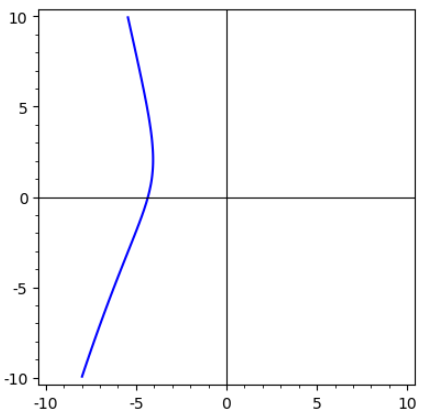
\includegraphics[width=0.4\textwidth]{conjuntzero.PNG}\\
    Conjunt \textit{$L_0$}
\end{center}

\begin{center}
    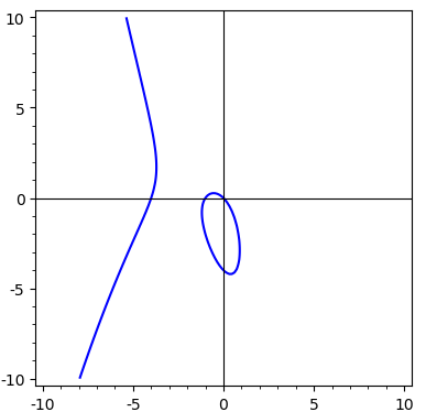
\includegraphics[width=0.4\textwidth]{conjuntcinc.PNG}\\
     Conjunt \textit{$L_5$}
\end{center}

\begin{center}
    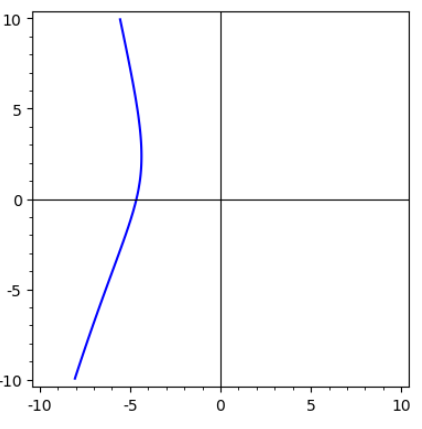
\includegraphics[width=0.4\textwidth]{conjuntsis.PNG}\\
     Conjunt \textit{$L_{-6}$}
\end{center}


\chapter{Exercici 6}
\section{Enunciat}
Considerem la funció que a cada punt de la circumferència centrada a l'origen i de radi 2 li assigna $\parallel \nabla f \parallel ^2$. On es troba el màxim? I el mínim?

\section{Procediment}
Considerem la circumferència centrada a l'origen i de radi 2:
$$\Omega := x^2 + y^2 = 4$$
Calculem el gradient de la funció $f(x,y) = x^{3} + 5x^{2} + 2xy + y^{2} + 4x + 4y + 5$:
$$\nabla f = (3x^2 + 10x + 2y + 4, 2x + 2y + 4)^2  $$
$$ \parallel \nabla f\parallel = \sqrt{(3x^2 + 10x + 2y + 4)^2 + ( 2x + 2y + 4)^2 }$$\\
Definim com $h(x,y) := \parallel \nabla f\parallel^2 = (3x^2 + 10x + 2y + 4)^2 + ( 2x + 2y + 4)^2$\\
Calculem el gradient de la funció $\Omega$: $\nabla \Omega = (2x, 2y)$\\
Calculem el gradient de $h$: $\nabla h(x,y)$
$$\nabla h(x,y) = ( 4(3x^2 + 10x + 2y + 4)(3x + 5) + 8x + 8y + 16, 12x^2 + 48 + 16y + 32)$$
Trobem les possibles solucions a partir del sistema format per $\Omega$ i $\nabla h= \nabla \Omega$:
\newline
$\left.
\begin{array}{rcl}
    4(3x^2 + 10x + 2y + 4)(3x + 5) + 8x + 8y + 16 & = & 2x\lambda\\
    12x^2 + 48 + 16y + 32 & = & 2y\lambda \\
    x^2 + y^2 & = & 4
\end{array}
\right\}$
\newline
Les solucions del sistema són:
\begin{itemize}
    \item $(x,y) = (0,-2) \longrightarrow h(x,y) = 0$
    \item $(x,y) = (1.987989886219975,0.2188507944092701) \longrightarrow h(x,y) = 1379.341929987197$
    \item $(x,y) = (-1.362133112856552,-1.464443045940843) \longrightarrow h(x,y) = 51.50913183573622$
    \item $(x,y) = (-1.880800727934486,0.6801385681293303) \longrightarrow h(x,y) = 10.595801545229449$
\end{itemize}
Finalment, el màxim i el mínim, respectivament, són: 
\begin{center}
    \fcolorbox{black}{white}{$(x,y) = (1.987989886219975,0.2188507944092701)$ i $(x,y) = (0,-2)$} 
\end{center}
\section{Solució}
El màxim és el punt $(x,y)=(1.987989886219975,0.2188507944092701)$.\\
El mínim és el punt $(x,y)=(0,-2)$.

\chapter{Exercici 7}
\section{Enunciat}
Si considerem la funció $h(x,y) = \frac{f(x,y)}{1-xy}$, determineu quin és el valor de $\frac{\partial ^{17} h }{\partial x^9 \partial y^8}$(0,0), $\frac{\partial ^{18} h }{\partial x^{10} \partial y^8}$(0,0) i $\frac{\partial ^{17} h }{\partial x^8 \partial y^9}(0,0)$

\section{Procediment}
$$h(x, y) = \frac{x^{3}+5x^{2}+2xy+y^{2}+4x+4y+5}{1-xy}$$
Desenvolupament per Taylor:
$$\frac{1}{1-x} = 1 + x + x^{2} + x^{3} + \cdots$$
$$\frac{1}{1-xy} = 1 + xy + xy^{2} + xy^{3} +  \cdots$$
Com f(x,y) és un polinomi, el polinomi de Taylor al punt (0,0) és:
\begin{equation*}
    (x^{3}+5x^{2}+2xy+y^{2}+4x+4y+5)\cdot (1 + xy + xy^2 + xy^3 + \cdots )
\end{equation*}
Calculem el valor de $\frac{\partial ^{17} h }{\partial x^9 \partial y^8}$(0,0) sabent que: 
\begin{equation*}
    \frac{1}{17!}\cdot\frac{17!}{9!8!}\cdot\frac{\partial ^{17} h }{\partial x^9 \partial y^8}(0,0) = \frac{1}{9!8!}\cdot\frac{\partial ^{17} h }{\partial x^9 \partial y^8}(0,0)
\end{equation*}
\newline\newline
Trobem ara el valor del coeficient del polinomi de taylor que té desembolupat $x^9y^8$ ja que sabem que el valor de l'expressió anterior serà la d'aquest coeficient.
\newline
Per tant ens interesa el producte  següent:
$$(x^{3}+5x^{2}+2xy+y^{2}+4x+4y+5)(x^8y^8)$$
Ja que d'aquí obtindrem $4x(x^8y^8) = 4x^9y^8$, per tant el valor del coeficient és $4$.\\
Calculem ara el valor de $\frac{\partial ^{17} h }{\partial x^9 \partial y^8}(0,0)$
$$\frac{1}{9!8!}\cdot\frac{\partial ^{17} h }{\partial x^9 \partial y^8}(0,0) = 4  \Rightarrow \frac{\partial ^{17} h }{\partial x^9 \partial y^8}(0,0) = 4\left(\frac{1}{9!8!}\right)^{-1}=4\cdot9!\cdot8! \Rightarrow $$
\begin{equation}
    \Rightarrow\fcolorbox{black}{white}{$ \frac{\partial ^{17} h }{\partial x^9 \partial y^8}(0,0) = 4\cdot9!\cdot8!$}
    \label{probabilitat cristall}
\end{equation}
Analogament, calculem els següents valors.
\newline
Valor de $\frac{\partial ^{18} h }{\partial x^{10} \partial y^8}(0,0):$
 $$\frac{1}{18!}\frac{18!}{10!8!}\frac{\partial ^18 h }{\partial x^10 \partial y^8}(0,0) =  \frac{1}{10!8!}\frac{\partial ^{18} h }{\partial x^{10} \partial y^8}(0,0)$$
El valor del coeficient del polinomi de Taylor és $5$ ja que s'obté del producte següent:
$$(x^{3}+5x^{2}+2xy+y^{2}+4x+4y+5)(x^8y^8)\rightarrow 5x^2(x^8y^8) = 5x^{10}y^8$$
Per tant,
$$\frac{\partial ^{17} h }{\partial x^{10} \partial y^8}(0,0) = 5 \left( \frac{1}{10!8!}\right)^{-1} = 5\cdot10!\cdot8!\Rightarrow$$
\begin{equation}
    \Rightarrow\fcolorbox{black}{white}{$ \frac{\partial ^{17} h }{\partial x^{10} \partial y^8}(0,0) = 5\cdot10!\cdot8!$}
    \label{probabilitat cristall}
\end{equation}
Valor de $\frac{\partial ^{17} h }{\partial x^{8} \partial y^9}(0,0):$\\
 $$\frac{1}{17!}\frac{17!}{8!9!}\frac{\partial ^{17} h }{\partial x^{8} \partial y^9}(0,0) =  \frac{1}{8!9!}\frac{\partial ^{17} h }{\partial x^{8} \partial y^9}(0,0)$$
El valor del coeficient del polinomi de Taylor és $4$ ja que s'obté del producte següent:
$$(x^{3}+5x^{2}+2xy+y^{2}+4x+4y+5)(x^8y^8)\rightarrow4y(x^8y^8) = 4x^{8}y^9$$ 
Finalment
$$\frac{1}{8!9!}\frac{\partial ^{17} h }{\partial x^{8} \partial y^9}(0,0) = 4 \left(\frac{1}{8!9!}\right)^{-1} = 4\cdot8!\cdot9! \Rightarrow$$
\begin{equation}
    \Rightarrow\fcolorbox{black}{white}{$ \frac{\partial ^{17} h }{\partial x^{8} \partial y^9}(0,0) = 4\cdot8!\cdot9!$}
    \label{probabilitat cristall}
\end{equation}


\section{Solució}
El valor de $\frac{\partial ^{17} h }{\partial x^9 \partial y^8}(0,0)$ és $4\cdot9!\cdot8!$.\\
El valor de $\frac{\partial ^{17} h }{\partial x^{10} \partial y^8}(0,0)$ és$ 5\cdot10!\cdot8!$.\\
El valor dede $\frac{\partial ^{17} h }{\partial x^{8} \partial y^9}(0,0)$ és $4\cdot8!\cdot9!$.


\chapter{Exercici 8}
\section{Enunciat}
Si considerem la funció $g(x,y,z) = f(3x^2-y^2+z^2, x+4y-z)$, quant val el gradient de $g$ en el punt $(2,-1,1)$?
\section{Procediment}
Calculem $ f(3x^2 - y^2 + z^2, x + 4y - z)$:
\[f(3x^2 - y^2 + z^2, x + 4y - z) = (3x^2 - y^2 + z^2)^3 + 5(3x^2 - y^2 + z^2)^2 + \]
\[+ 2(3x^2 - y^2 + z^2)(x + 4y - z)  + (x + 4y - z)^2+12x^2 - 4y^2 + 4z^2 + 4x + 16y - 4z + 5\]
Calculem el gradient de $g(x,y,z)$: $\nabla g(x,y,z)$
$$\nabla g(x,y,z)=
\left(
\begin{array}{c}
     \scriptstyle
     18(3x^2 - y^2 + z^2)^2x + 60(3x^2 - y^2 + z^2)x + 12(x + 4y - z)x + 6x^2 - 2y^2 + 2z^2 + 26x + 8y - 2z + 4  \\
      \scriptstyle
     -6(3x^2 - y^2 + z^2)^2y + 24x^2 - 20(3x^2 - y^2 + z^2)y - 4(x + 4y - z)y - 8y^2 + 8z^2 + 8x + 24y - 8z + 16 \\
      \scriptstyle
     (3x^2 - y^2 + z^2)^2z - 6x^2 + 2y^2 + 20(3x^2 - y^2 + z^2)z + 4(x + 4y - z)z - 2z^2 - 2x - 8y + 10z - 4
\end{array}
\right)$$
\newline
Per últim, substituix (x, y, z) per (2, -1, 1): (6622, 1188, 1078)\\
També vam fer el càlcul amb \textit{SageMath}:
\begin{verbatim}
    g(x,y,z) = f(3x^2 - y^2 + z^2, x + 4y - z)
    g.gradient()(2, -1, 1)
\end{verbatim}

\section{Solució}
El gradient de $g(x,y,z)$ en el punt $(2,1,-1)$ és $(6622, 1188, 1078)$.


\chapter{Exercici 9}
\section{Enunciat}
Considereu ara el conjunt de punts on el vostre polinomi és igual a $x^3+12$. Parametritzeu aquesta corba i calculeu, aproximadament, la seva longitud.
\section{Procediment}
Escribim la equació en forma d'elipse:
$$5x^2+2xy+y^2+4x+4y-7=0 \Rightarrow \frac{(x+y+2)^2} {(\sqrt{11})^2}+\frac{(x)^2}{(\frac{\sqrt{11}}{2})^2}=1 $$
Parametrizem la corba de la forma:
$$\gamma(t) = (x(t), y(t))$$
On:
$$\left.
\begin{array}{ccc}
     x(t) & = & a\cos{t} \\
     y(t) & = & b\sin{t} \\
\end{array}\right\}
\Longrightarrow
\left.
\begin{array}{ccc}
    x(t) & = & \frac{\sqrt{11}}{2}\cos{t} \\
    x(t) + y(t)+ 2 & = & \sqrt{11}\sin{t} 
\end{array}\right\}
\Longrightarrow$$
$$\Longrightarrow\left.
\begin{array}{ccc}
    x(t) & = & \frac{\sqrt{11}}{2}\cos{t} \\
    y(t) & = &  \sqrt{11}\sin{t} -2 - \frac{\sqrt{11}}{2}\cos{t}
\end{array}\right\} \Longrightarrow$$

$$\Longrightarrow \gamma(t) = \left(\frac{\sqrt{11}}{2}\cos{t},-2+\sqrt{11}\sin{t}-\frac{\sqrt{11}}{2}\cos{t}\right)$$
\newpage
Calculem la longitud:

$$L(\gamma(t)) = \int_{0}^{2\pi} \sqrt{||\gamma'(t)||}dt$$

$$L(\gamma(t)) = \int_{0}^{2\pi} \sqrt{\left(-\frac{\sqrt{11}}{2}\sin{t}\right)^2+\left(\sqrt{11}\cos{t}+\frac{\sqrt{11}}{2}\sin{t}\right)^2} dt \approx 17.3092395644920 u $$
\begin{center}
    \fcolorbox{black}{white}{$L(\gamma(t))=17.3092395644920 u$}
\end{center}


\section{Solució}
La Longitud de la corba  és $17.3092395644920$ unitats.
\begin{center}
    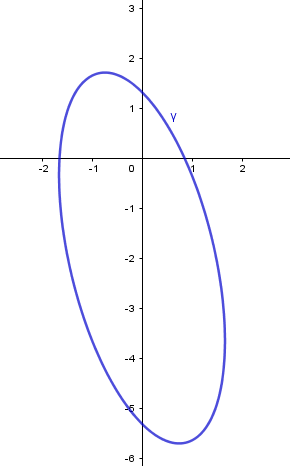
\includegraphics{elipse.PNG}
\end{center}


\chapter{Exercici 10}
\section{Enunciat}
Determineu, fent servir el teorema de Green, l'àrea de la regió limitada per la corba anterior.
\section{Procediment}
Sigui $\overrightarrow{F}(x,y)=(-y,x)$ la funció del camps vectorial i $\Omega$ la regió delimitada per la corba $\varphi$, essent aquesta l'el·lipse de l'exercici anterior, $\varphi(t)= \left(\frac{\sqrt{11}}{2}\cos{t},-2+\sqrt{11}\sin{t}-\frac{\sqrt{11}}{2}\cos{t}\right)$, podem calcular l'àrea mitjançant la fórmula:
$$Àrea(\Lambda)= \frac{1}{2} \oint_{\gamma} \overrightarrow{\digamma} \text{,     sabent que:     } \oint_C \overrightarrow{\digamma} = \int_{a}^{b} \overrightarrow{\digamma}(\gamma(t)) \cdot \gamma'(t)dt \text{ ; on } t \in [a,b]$$
% Sabem que la integral de línia d'un camp vectorial $\overrightarrow{\digamma}$ sobre una corba $\gamma$ parametritzada amb $t \in [a,b]$ és:
% $$\int_C \overrightarrow{\digamma} = \int_{a}^{b} \overrightarrow{\digamma}(\gamma(t)) \cdot \gamma'(t)dt$$
Per tant, en el nostre cas, calculem la integral de linia del camp vectorial $F$ sobre la corba $\varphi$ per a $t \in [0,2\pi]$

 \begin{gather*}
 \bigintssss_{0}^{2\pi}
     \left( 2-\sqrt{11}\sin{t}+\frac{\sqrt{11}}{2}\cos{t}, \frac{\sqrt{11}}{2}\cos{t} \right) \left( -\frac{\sqrt{11}}{2}\sin{t}, \sqrt{11}\cos{t}+\frac{\sqrt{11}}{2}\sin{t}\right) dt =
 \end{gather*}
\begin{gather*}
    = \! \bigintssss_0^{2\pi} \! \left(\frac{1}{4}\sqrt{11}\left(2\sqrt{11}\cos{t} + \sqrt{11}\sin{t}\right)\cos{t} - \frac{1}{4}\sqrt{11}\left(\sqrt{11}\cos{t} - 2\sqrt{11}\sin{t} + 4\right)\sin{t}\right) \! dt\! =
\end{gather*}
\begin{equation*}
    = 11\pi \Rightarrow \bigointssss_0^{2\pi} \overrightarrow{F} = 11\pi \Rightarrow \fcolorbox{black}{white}{$Area(\Omega)=\frac{11\pi}{2} u^2.$}
\end{equation*}




\section{Solució}
L'àrea de la regió limitada per la corba anterior és $\frac{11\pi}{2} u^2$ .


%\Rightarrow \frac{(x+y)^2 +4(x^2+x+y)}{7}=1 $$
%$$\frac{(x+y)^2 +4(x^2+x+y)}{7}=1 \Rightarrow \frac{(x+y+2)^2 +4x^2-4}{7}=1\Rightarrow $$

%$$\frac{(x+y+2)^2 +4x^2}{11}=1$$





\end{document}
